\documentclass{article}

\usepackage[margin=1in]{geometry}
\usepackage[utf8]{inputenc}
\usepackage{amsmath}
\usepackage{tikz}
\usepackage{sectsty}
\usetikzlibrary{automata,positioning}

\title{Homework \#2A second part}
\date{April 21th 2020}
\author{Zoe Sadeghi,\\University of Washington, Tacoma}

\sectionfont{\fontsize{12}{15}\selectfont}

\begin{document}

\maketitle

\section{Problem 4}

\paragraph{Part a}
\begin{center}
    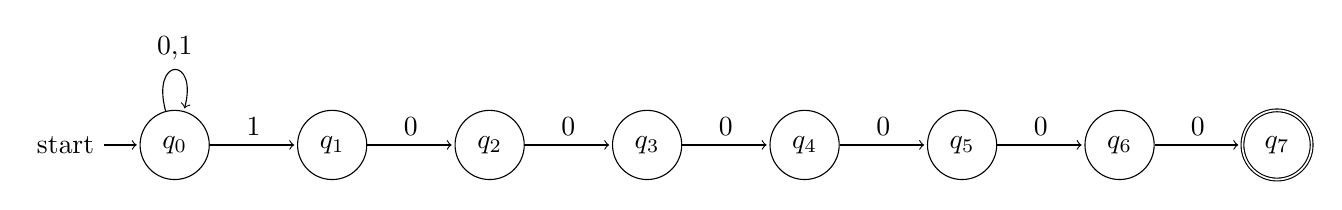
\begin{tikzpicture}[shorten >=1pt,node distance=2cm,on grid,auto] 
        \node[state,initial] (q_0)   {$q_0$}; 
        \node[state] (q_1) [right=of q_0] {$q_1$}; 
        \node[state] (q_2) [right=of q_1] {$q_2$}; 
        \node[state] (q_3) [right=of q_2] {$q_3$};
        \node[state] (q_4) [right=of q_3] {$q_4$};
        \node[state] (q_5) [right=of q_4] {$q_5$};
        \node[state] (q_6) [right=of q_5] {$q_6$};
        \node[state, accepting] (q_7) [right=of q_6] {$q_7$};
        \path[->] 
        (q_0) edge [loop above] node {0,1} (q_0)
        (q_0) edge node {1} (q_1)
        (q_1) edge node {0} (q_2)
        (q_2) edge node {0} (q_3)
        (q_3) edge node {0} (q_4)
        (q_4) edge node {0} (q_5)
        (q_5) edge node {0} (q_6)
        (q_6) edge node {0} (q_7);
    \end{tikzpicture}
\end{center}


\paragraph{Part b}
\begin{enumerate}

\item It is trivially observable that $(s,w) \vdash^1_M (q_{000000a},\varepsilon)$ where $w=a$, due to the definition of $\delta$.

\item For $|w| = 2, (s,w) \vdash^2_M (q_y, \varepsilon) \equiv (s, w) \vdash^1_M (q_{w_1}, w_2) \vdash^1_M (q_y, \varepsilon)$ and according to $1$ above, $q_{w_1}$ is in the form of $q_{000000a}$, which means $q_{w_2}$ will be in the form of $q_{00000ab}$ where $w=ab$ and it follows that $(s,w) \vdash^{|w|}_M (q_y, \varepsilon) \Rightarrow y= 0^k w , k=7-|w|$

\item For ${|w|} \geq 7 : (s, w) \vdash^*_M (q_y, \varepsilon)$ where $w \in \Sigma^*y$ and $|y|= 7$ , then for $u=w.a$ with $a \in \Sigma$ , we will have $(s, u) \vdash^{|w|}_M (q_y, a)$. In this case, iff $y \in \Sigma1\Sigma^5$, due to the definition of $\delta$ , we will have $(q_y, a) \vdash^1_M (q_v, \varepsilon)$ where $v \in 1\Sigma^6$, or, in other words, $q_v \in F$.

\end{enumerate}


\paragraph{bonus}

Let's assume we have $M'$ where $|M'| < 2^7$ and $L(M') = L$. Given $W \subset L$ where $W = \{ w| |w| \geq 7 \}$, since $|W| \geq 2^7$, according to the pidgeon-hole principle, there are at least words $w_1$ and $w_2 \in W$ where the seventh symbol from the last for them are different, which fall to the same state $q_i$ of $M'$ . Based on our definition, one of $w_1$ and $w_2$ is in $L$, however $q_i$ cannot be both an accepting, and a non-accepting state. Therefore, no such $M'$ exists where $|M'| < 2^7$.

\end{document}  

